\documentclass[sigconf]{acmart}
\usepackage{algorithm}
\usepackage{algpseudocode}
\usepackage{bm}
\usepackage{bbm}

\settopmatter{printacmref=false} % Removes citation information below abstract
\renewcommand\footnotetextcopyrightpermission[1]{}
\newcommand{\sign}{\text{sign}}
\pagestyle{plain} % removes running headers

%%
%% \BibTeX command to typeset BibTeX logo in the docs
\AtBeginDocument{%
  \providecommand\BibTeX{{%
    Bib\TeX}}}

\setcopyright{None}

\settopmatter{printacmref=false}

\begin{document}

\title{Robust Principal Component Analysis on Graphs}

\author{Sofiane Ezzehi}
\affiliation{%
  \institution{École Normale Supérieure Paris-Saclay \\ École des Ponts ParisTech}
  \country{}
}
\email{sofiane.ezzehi@eleves.enpc.fr}

\author{Alexandre Lutt}
\affiliation{%
  \institution{École Normale Supérieure Paris-Saclay \\ École des Ponts ParisTech}
  \country{}
}
\email{alexandre.lutt@eleves.enpc.fr}

\begin{teaserfigure}
  \center
  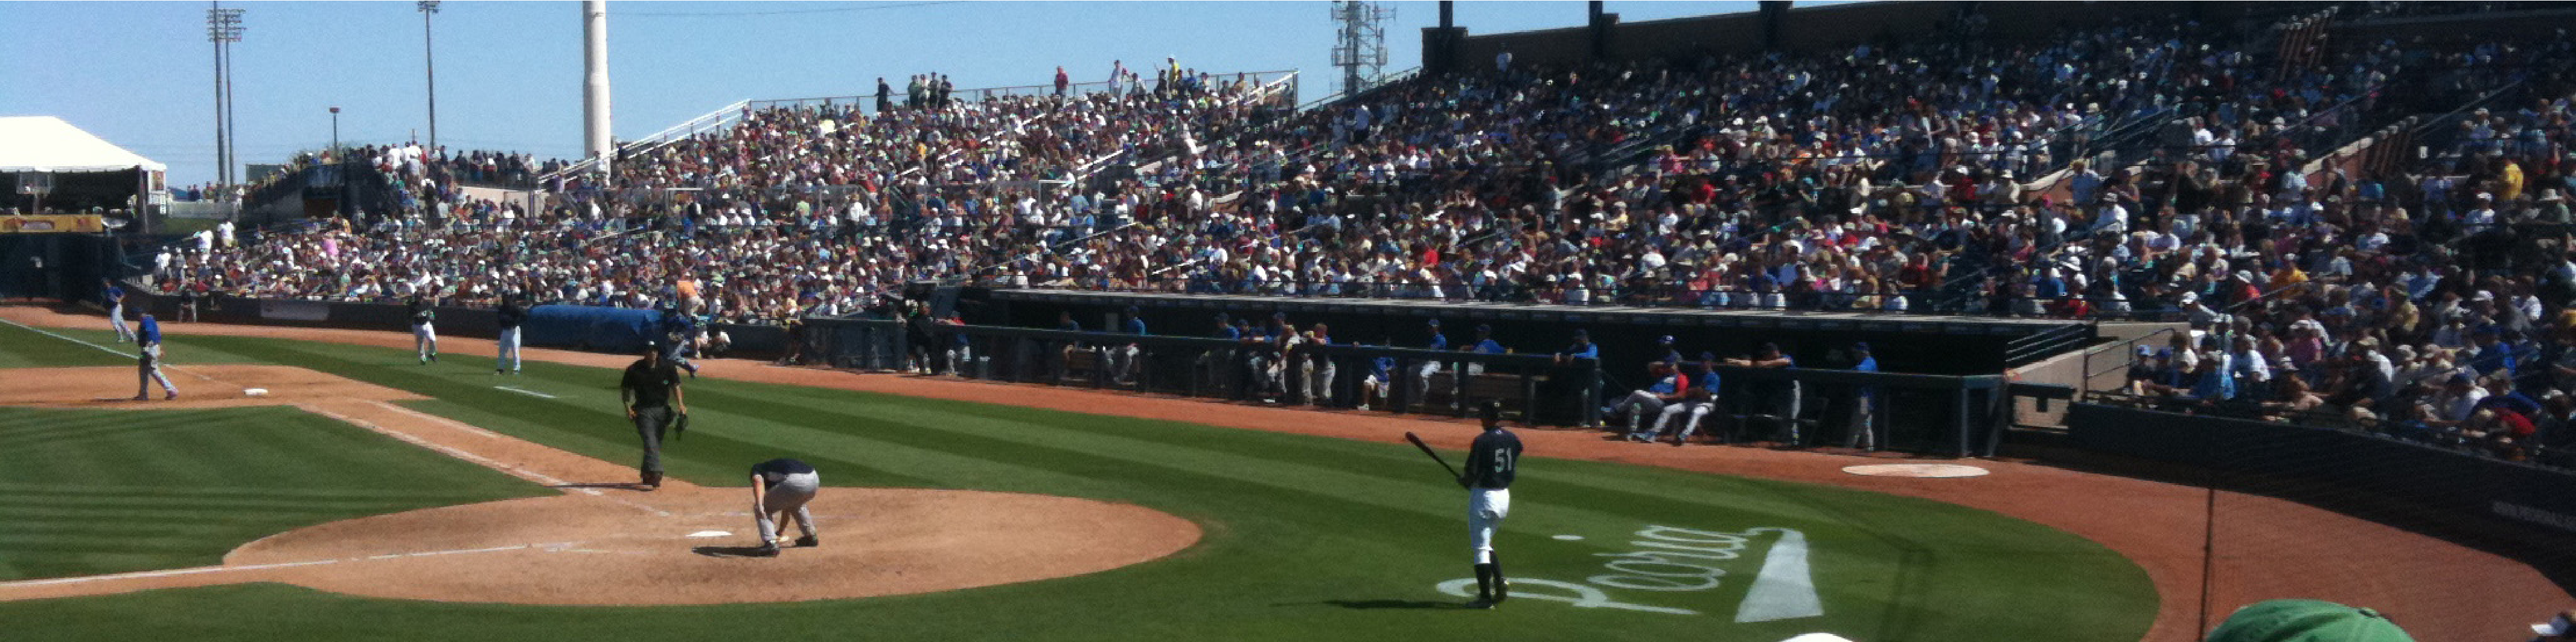
\includegraphics[width=15cm, height=7cm]{sampleteaser}
  \caption{Low-rank reconstruction of corrupted images using the proposed method of~\cite{main_paper}.}
  \Description{Low-rank reconstruction of corrupted images.}
  \label{fig:teaser}
\end{teaserfigure}

\maketitle
\pagestyle{plain}

\section{Abstract}

Principal Component Analysis (PCA) is a very popular method for dimensionality reduction, and is used by thousands accross the world to provide 2D or 3D visualisations and insights about high-dimension data. It is used in a variety of different fields, such as image processing, finance, biology, and computer vision, to name only a few of them.
In this work, we present a benchmark of different variants of PCA, which aim to tackle some of the issues of the original PCA algorithm that prevent it from being used in many real-life situations. 

\section{Introduction}

As mentionned in the abstract, PCA is a useful tool for dimensionnality reduction. More specifically, given a matrix $X \in \mathbb{R}^{n \times p}$, it solves the following optimization problem:

\begin{equation*}
  \begin{aligned}
  & \underset{L \in \mathbb{R}^{n \times p}}{\min}
  & & ||X - L||_F^2 \\
  & \text{subject to}
  & & rank(L) \leqslant k \\
  \end{aligned}
\end{equation*}

where $k$ is an integer parameter of the algorithm. It can be shown that this problem actually has a closed-form solution given by the first $k$ principal components of $X$.

However, the main drawback of PCA is that it is very sensitive to noise, corrupted data and outliers and thus cannot be used in many real-world applications.
The sensitivity to noise has been partially solved by the introduction of a robust variant of PCA, RPCA~\cite{rpca_paper}. However, this algorithm is very slow on large datasets, which makes it impractical for many applications. 
This motivated the introduction of another PCA variant called GLPCA~\cite{glpca_paper} which uses graph Laplacian regularization to improve the robustness of the algorithm while keeping the computational cost low.
Finally, a third variant of PCA similar to the previous ones has been proposed by the authors of~\cite{main_paper} to improve the robustness of the algorithm while keeping the computational cost low.

This project aims to provide a simple and efficient implementation of those main variants of the PCA algorithm, as well as a benchmark of those methods on different tasks (clustering and low-rank recovery for corrupted data on real-life and artificial datsets).

\section{Algorithms}

In this section, we are going to present the algorithms we implemented and compared for the benchmark.

\begin{itemize}
  \item \textbf{Classsical PCA}: We used Scikit-Learn implementation of PCA, which computes the SVD of $X$ and returns the first $k$ principal components.
  \item \textbf{RPCA}: We implemented (see algorithm~\ref{alg:rpca}) the algorithm described in~\cite{rpca_paper} using the ADMM (Alternating Direction Method of Multipliers) and following as closely as possible the pseudo-code provided in the paper.
  This algorithm solves the following optimization problem:

  \begin{equation*}
    \begin{aligned}
    & \underset{L, S \in \mathbb{R}^{n \times p}}{\min}
    & & ||L||_* + \lambda ||S||_1 \\
    & \text{subject to}
    & & L + S = X \\
    \end{aligned}
  \end{equation*}

  where $||.||_*$ is the nuclear norm and $||.||_1$ is the $\ell_1$ norm. This problem is solved iteratively by alterining phases of optimization over $L$ and over $S$.
  
  \item \textbf{GLPCA}: We also implemented (see algorithm~\ref{alg:glpca}) the algorithm described in~\cite{glpca_paper} using the closed-form solution proved in the original paper.
  
  This algorithm solves the following optimization problem:

  \begin{equation*}
    \begin{aligned}
    & \underset{Q, U \in \mathbb{R}^{n \times k}}{\min}
    & & ||X - UQ^T||_F^2 + \alpha Tr(Q^T (D-W) Q) \\
    & \text{subject to}
    & & Q^TQ = I \\
    \end{aligned}
  \end{equation*}

  Where $W$ is the adjacency matrix of the graph $\mathcal{G}$, $D$ is the degree matrix of $\mathcal{G}$, and $\alpha$ is a hyperparameter of the algorithm. In pratice, we followed the pseudo-code provided in paper~\cite{glpca_paper} and used the closed-form solution obtained when reformulating the problem using $\alpha = \dfrac{\beta}{1 - \beta} \dfrac{\lambda_n}{\xi_n}$ (where $\lambda_n$ and $\xi_n$ are respectively the maximum eigenvalues of $X^TX$ and $D-W$) and differentiating the objective function with respect to $Q$ and $U$.

  \item \textbf{RGLPCA}: We also implemented (see algorithm~\ref{alg:rglpca}) the robust version of the previous algorithm also mentionned in~\cite{glpca_paper}. This algorithm solves the following optimization problem:
  
  \begin{equation*}
    \begin{aligned}
    & \underset{Q, U \in \mathbb{R}^{n \times k}}{\min}
    & & ||X - UQ^T||_{2, 1} + \alpha Tr(Q^T (D-W) Q) \\
    & \text{subject to}
    & & Q^TQ = I \\
    \end{aligned}
  \end{equation*}

  where $||.||_{2, 1}$ is the $\ell_{2, 1}$ norm defined by $||A||_{2, 1} = \sum\limits_{j=1}^n \sqrt{\sum \limits_{i=1}^p A_{ij}^2}$. This problem is solved using the ADMM algorithm, following the pseudo-code provided in the paper.
  
  \item \textbf{Proposed PCA}: Finally, we implemented (see algorithm~\ref{alg:our_pca}) the algorithm described in~\cite{main_paper} which claims to be more robust than the previous ones while keeping the computational cost low. This algorithm solves the following optimization problem:
  
  \begin{equation*}
    \begin{aligned}
    & \underset{L, S \in \mathbb{R}^{n \times p}}{\min}
    & & ||L||_* + \lambda ||S||_1 + \gamma Tr(L \phi L^T) \\
    & \text{subject to}
    & & X = L + S \\
    \end{aligned}
  \end{equation*}

  Where $\phi$ is the graph Laplacian of $\mathcal{G}$ and $\gamma$ is a hyperparameter of the algorithm. As the previous methods, it uses the ADMM algorithm to solve this problem by alternating phases of optimization over $L$ and over $S$.

\end{itemize}
 
In order to make notations more concise, we will define the following shrinkage and singular value tresholding operators (defined on the space of square matrices):

\begin{equation*}
  \begin{cases}
    \mathcal{S}_{\tau}(\mathbf{Z}) = \sign{(\mathbf{Z})} \times \max{(\mathbf{0}, |\mathbf{Z}| - \tau \mathbf{I})} \\
      \mathcal{D}_{\tau}(\mathbf{Z}) = \mathbf{U} \mathcal{S}_{\tau}(\mathbf{\Sigma}) \mathbf{V}^T \text{ with } \mathbf{Z} = \mathbf{U} \mathbf{\Sigma} \mathbf{V}^T
  \end{cases}
\end{equation*}

\begin{algorithm}
  \caption{RPCA algorithm}\label{alg:rpca}
  \begin{algorithmic}
      \Require $\mathbf{X} \in \mathbb{R}^{m \times n}$, $\varepsilon$, $n_{iter}$
      
      \State $\lambda \gets \frac{1}{\sqrt{\max(m, n)}}$
      \State $\mu \gets \frac{\max(m, n)}{4 \times ||\mathbf{X}||_1}$
      \State $\mathbf{S} \gets \mathbf{0}$
      \State $\mathbf{Y} \gets \mathbf{0}$
      
      \For{$i = 1$ \textbf{to} $n_{iter}$}
          \State $\mathbf{L} \gets \mathcal{D}_{\mu}(\mathbf{X} - \mathbf{S} + \frac{1}{\mu} \mathbf{Y})$
          \State $\mathbf{S} \gets \mathcal{S}_{\frac{\lambda}{\mu}} (\mathbf{X} - \mathbf{L} + \frac{1}{\mu} \mathbf{Y})$ 
          \State $\mathbf{Y} \gets \mathbf{Y} + \mu(\mathbf{X} - \mathbf{L} - \mathbf{S})$
          \If{$||\mathbf{X} - \mathbf{L} - \mathbf{S}||_{F} \leqslant \varepsilon$}
              \State break\
          \EndIf
      \EndFor
      
      \State \Return $\mathbf{L}$, $\mathbf{S}$
  \end{algorithmic}
  \end{algorithm}
  
  \begin{algorithm}
  \caption{GLPCA algorithm}\label{alg:glpca}
  \begin{algorithmic}
      \Require $\mathbf{X} \in \mathbb{R}^{m \times n}$, $\mathcal{G}$,  $\beta$
      
      \State $\mathbf{W} \gets adj(\mathcal{G})$
      \State $\mathbf{D} \gets diag(\{d_1, d_2, ..., d_{n_{\text{nodes}}}\})$
      \State $\mathbf{L} \gets \mathbf{D} - \mathbf{W}$
      
      \State $\lambda_n \gets \Re(\max(eigenval(\mathbf{X}^T\mathbf{X}))$
      \State $\xi_n \gets \Re(\max(eigenval(\mathbf{L}))$
      
      \State $\mathbf{G}_{\beta} \gets (1 - \beta)(\mathbf{I} - \frac{1} {\lambda_n}\mathbf{X}^T\mathbf{X}) + \frac{\beta}{\xi_n}\mathbf{L}$
      
      \State $\mathbf{Q} \gets \Re{(eigenvect(\mathbf{G}_{\beta}))}$
      \State $\mathbf{U} \gets \mathbf{XQ}$
      
      \State \Return $\mathbf{Q}$, $\mathbf{U}$
  \end{algorithmic}
  \end{algorithm}
  
  
  \begin{algorithm}[H]
  \caption{RGLPCA algorithm}\label{alg:rglpca}
  \begin{algorithmic}
      \Require $\mathbf{X} \in \mathbb{R}^{m \times n}$, $\mathcal{G}$, $\beta$, $k$, $\rho$, $n_{iter}$
      
      \State $\mathbf{X}_0 \gets \mathbf{X}$
      \State $\beta_0 \gets \beta$
      
      \State $\mathbf{E} \gets \bm{1}$
      \State $\mathbf{C} \gets \bm{1}$
      \State $\mu \gets 1$
      
      \State $\mathbf{W} \gets adj(\mathcal{G})$
      \State $\mathbf{D} \gets diag(\{d_1, d_2, ..., d_{n_{\text{nodes}}}\})$
      \State $\mathbf{L} \gets \mathbf{D} - \mathbf{W}$
      
      \State $\xi \gets \Re(max(eigenval(\mathbf{X}_0^T \mathbf{X}_0)))$
      
      \For{$i = 1$ \textbf{to} $n_{iter}$}
          \State $\mathbf{X}_i \gets \mathbf{X} - \mathbf{E} - \frac{1}{\mu}\mathbf{C}$
          \State $\lambda \gets \Re(\max(eigenval(\mathbf{X}_i^T \mathbf{X}_i)))$
      
          \State $\alpha \gets \frac{2 \beta_0 \lambda}{\mu (1 - \beta_0)\xi}$
          \State $\beta \gets \frac{\alpha \xi}{\lambda + \alpha \xi}$
      
          \State $\mathbf{Q}, \mathbf{U} \gets GLPCA(\mathbf{X}, \mathcal{G}, \beta, k)$
      
          \State $\mathbf{A} \gets \mathbf{X}_k - \mathbf{UQ}^T - \frac{1}{\mu} \mathbf{C}$
          \State $\mathbf{a} \gets (||\mathbf{A}_1||_2, ||\mathbf{A}_2||_2, ..., ||\mathbf{A}_m||_2)$
          \State $\mathbf{E} \gets \mathcal{S}_{\frac{1}{\mu}}(\mathbf{a})$
          \State $\mathbf{C} \gets \mathbf{C} + \mu(\mathbf{E} - \mathbf{X} - \mathbf{UQ}^T)$
          \State $\mu \gets \rho \mu$
          
      \EndFor
      
      \State \Return $\mathbf{Q}$, $\mathbf{U}$, $\mathbf{E}$
  \end{algorithmic}
  \end{algorithm}
  
  
  \begin{algorithm}[H]
  \caption{Proposed PCA algorithm}\label{alg:our_pca}
  \begin{algorithmic}
      \Require $\mathbf{X} \in \mathbb{R}^{p \times n}$, $\mathcal{G}$, $n_{iter}$, $\gamma$, $\varepsilon$
      
      \State $\mathbf{A} \gets adj(\mathcal{G})$
      \State $\mathbf{D} \gets diag(\{d_1, d_2, ..., d_{n_{\text{nodes}}}\})$
      
      \State $\bm{\phi} \gets D^{-\frac{1}{2}} A D^{-\frac{1}{2}} $
      
      \State $\lambda \gets \frac{1}{\sqrt{\max(p, n)}}$
      \State $\mathbf{L} \gets random(p, n)$
      \State $\mathbf{W} \gets random(p, n)$
      \State $\mathbf{S} \gets random(p, n)$
      
      \State $r_1 \gets 1$
      \State $r_2 \gets 1$
      
      \State $\mathbf{Z}_1 \gets \mathbf{X} - \mathbf{L} - \mathbf{S}$
      \State $\mathbf{Z}_2 \gets \mathbf{W} - \mathbf{L}$
      
      \For{$i = 1$ \textbf{to} $n_{iter}$}
          \State $\mathbf{H}_1 \gets \mathbf{X} - \mathbf{S} + \frac{1}{r_1}\mathbf{Z}_1$
          \State $\mathbf{H}_2 \gets \mathbf{W} + \frac{1}{r_2}\mathbf{Z}_2$
          \State $\mathbf{H} \gets \frac{1}{r_1 + r_2} (r_1 \mathbf{H}_1 + r_2 \mathbf{H}_2)$
          \State $\mathbf{L} \gets \mathcal{D}_{\frac{2}{r_1 + r_2}}(\mathbf{H})$
      
          \State $\mathbf{S} \gets \mathcal{S}_{\frac{\lambda}{r_1}}(\mathbf{X} - \mathbf{L} + \frac{1}{r_1}\mathbf{Z}_1)$
          \State $\mathbf{W} \gets r_2 (\gamma \bm{\phi} + r_2 \mathbf{I})^{-1}(L - \frac{1}{r_2}Z_2)$
          
          \State $\mathbf{Z}_1 \gets \mathbf{Z}_1 + r_1(\mathbf{X} - \mathbf{L} - \mathbf{S})$
          \State $\mathbf{Z}_2 \gets \mathbf{Z}_2 + r_2(\mathbf{W} - \mathbf{L})$
      
          \If{$||\mathbf{X} - \mathbf{L} - \mathbf{S}||_{F} \leqslant \varepsilon$}
              \State break\
          \EndIf
      
      \EndFor
      
      \State \Return $\mathbf{L}$, $\mathbf{S}$
  \end{algorithmic}
  \end{algorithm}




\section{Experimental setup}




\section{Results}




\section{Limitations}




\section{Conclusion}




%%
%% The next two lines define the bibliography style to be used, and
%% the bibliography file.
\bibliographystyle{ACM-Reference-Format}
\bibliography{bib}

\end{document}
\endinput